\documentclass{article}

\usepackage{tikz}

\begin{document}

\begin{center}
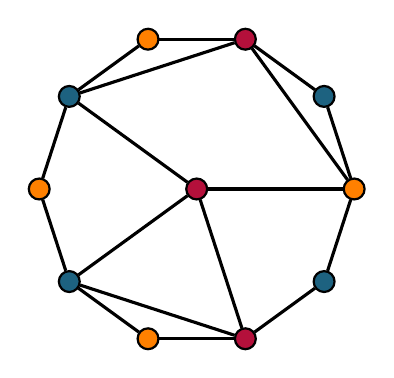
\begin{tikzpicture}[every node/.style={circle,thick,draw,scale=0.8}, line width=0.04cm]
    \node[fill = {rgb:red,255;green,22;blue,84}] (K) at (0:0) {};

    \node[fill = orange] (E) at (0:2) {};
    \node[fill = {rgb:red,36;green,123;blue,160}] (J) at (36:2) {};
    \node[fill = {rgb:red,255;green,22;blue,84}] (A) at (72:2) {};
    \node[fill = orange] (F) at (108:2) {};
    \node[fill = {rgb:red,36;green,123;blue,160}] (B) at (144:2) {};
    \node[fill = orange] (G) at (180:2) {};
    \node[fill = {rgb:red,36;green,123;blue,160}] (C) at (216:2) {};
    \node[fill = orange] (H) at (252:2) {};
    \node[fill = {rgb:red,255;green,22;blue,84}] (D) at (288:2) {};
    \node[fill = {rgb:red,36;green,123;blue,160}] (I) at (324:2) {};

    \draw (A) -- (B);
    \draw (A) -- (F);
    \draw (F) -- (B);
    \draw (B) -- (G);
%    \draw (B) -- (C);
    \draw (G) -- (C);
    \draw (C) -- (H);
    \draw (C) -- (D);
    \draw (H) -- (D);
    \draw (D) -- (I);
%    \draw (D) -- (E);
    \draw (I) -- (E);
    \draw (E) -- (A);
    \draw (E) -- (J);
    \draw (J) -- (A);
%    \draw (K) -- (A);
    \draw (K) -- (B);
    \draw (K) -- (C);
    \draw (K) -- (D);
    \draw (K) -- (E);
\end{tikzpicture}
\end{center}

\end{document}